\documentclass[notitlepage]{math}
\usepackage{lipsum}
\usepackage{tikz}
\usepackage{enumitem}
\usetikzlibrary{patterns,positioning, decorations, decorations.pathreplacing}
\newcommand*\circled[1]{\tikz[baseline=(char.base)]{
            \node[shape=circle,draw,inner sep=2pt] (char) {#1};}}
\title{Linear Maps Chap. 12} %Titre du fichie
\author{FireGhost} %Auteur du fichier

\begin{document}
\titre{Chapter 12: Linear Maps} %Titre du fichier .pdf
\UE{Linear Maps} %Nom de la UE

\fairetitre
\fairemarges
% subsubsubsection
\setcounter{secnumdepth}{4}

\titleformat{\paragraph}
{\normalfont\normalsize\bfseries}{\theparagraph}{1em}{}
\titlespacing*{\paragraph}
{0pt}{3.25ex plus 1ex minus .2ex}{1.5ex plus .2ex}

%
\section{General approach}
\subsection{Definition}
Let $E,F$ two $\mathbb{K}-VS$, and $f$ a mapping from $E$ to $F$.
We say that $f$ is a linear (or $f$ is a linear map) if:
\[ \forall (\alpha,X,Y)\in \mathbb{K} \times E \times E, f(\alpha \cdot X + Y) = \alpha \cdot f(X) + f(Y)\]
\[  \Longleftrightarrow  \]
\[  \forall (\alpha,\beta,X,Y)\in \mathbb{K} \times \mathbb{K} \times E \times E, f(\alpha \cdot X + \beta \cdot Y) = \alpha \cdot f(X) + \beta \cdot f(Y)\]
\subsection{Notation}
We denote $L(E,F)$ the set of all linear maps from $E$ to $F$.
\subsection{Specific Linear Maps}
\subsubsection{Definition}
\begin{enumerate}
    \item Let $f \in \mathcal{L}(E,F)$: we say $f$ is an endomorphism if $E = F$ we then denote $\mathcal{L}(E)$ the set of all endomorphism of $E$. 
    \item Let $f \in \mathcal{L}(E,F)$: we say $f$ is an isomorphism if $f$ is bijective.
    \item Let $f \in \mathcal{L}(E,F)$: we say $f$ is an automorphism if $f$ is an endomorphism and an isomorphism. ($E = F$ and bijective)
\end{enumerate}
\subsection{Necessary Condition}
\[ f \in \mathcal{L}(E,F) \Longrightarrow f(0_E)=0_F\]
\subsubsection{Proof}
\begin{minipage}{0.4\linewidth}
    \[\text{Let } X \in E\]
    \[f(0_E) = f(0_E \times X)\]
    \[f(0_E) = 0_F \times f(X)\]
    \[f(0_E) = 0_F\]
\end{minipage}
\hfill\vline\hfill
\begin{minipage}{0.49\linewidth}
    \[\text{Let } X \in E\]
    \[f(0_E) = f(X - X) \]
    \[f(0_E) = f(X) - f(X) \]
    \[f(0_E) = 0_F\]
\end{minipage}

\newpage
\section{Kernel and Images}
\subsection{Definition}
Let $E$ and $F$ two $\mathbb{K}-VS$ and $f \in \mathcal{L}(E,F)$. Then:

\begin{enumerate}
    \item We call kernel of $f$ and denote $Ker(f)$ the subset of $E$ defined as follows: 
    \[ Ker(f) = \{X \in E, f(X) = 0_F\} = f^{-1}(\{0_F\})\]
    \textit{Note: $f^{-1}()$ is NOT the inverse of $f$ beacause $f$ is not necessarily bijective.}
    \item We call image of $f$ and denote $Im(f)$ the subset of $F$ defined as follows:
    \[ Im(f) = \{f(X), X \in E\}=\{Y \in F, \exists X \in E, f(X) = Y\}\]
\end{enumerate}
\subsection{Graphics representation}
    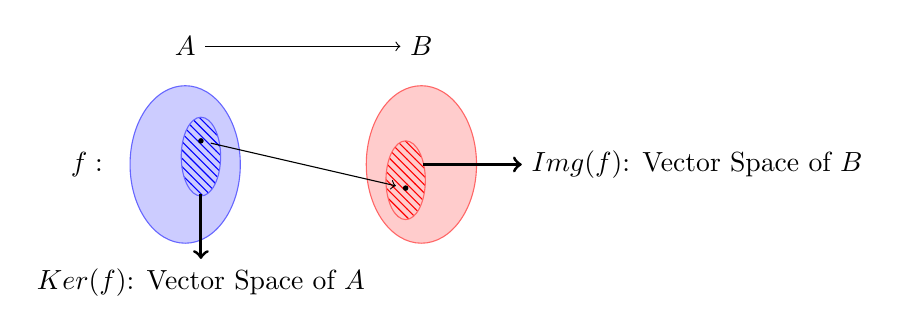
\begin{tikzpicture}
        % draw the sets
        \filldraw[fill=blue!20, draw=blue!60] (-1.5,0) ellipse (0.7cm and 1cm);
        \filldraw[draw=blue!60, pattern = north west lines, pattern color=blue] (-1.3,0.1) ellipse (0.25cm and 0.5cm) ;
        \filldraw[fill=red!20, draw=red!60] (1.5,0) ellipse (0.7cm and 1cm);
        \filldraw[draw=red!60, pattern = north west lines, pattern color=red] (1.3,-0.2) ellipse (0.25cm and 0.5cm);

        % the texts
        \node at (-2.75,0) {$f:$};
        \node (A) at (-1.5,1.5) {$A$};
        \node (B) at (1.5,1.5) {$B$};

        % the points in the sets (here I just create nodes to use them later on to position
        % the circles and the arrows
        \node (kerf1) at (-1.3,-0.25) {};
        \node (kerf2) at (-1.3,-1.5) {$Ker(f)$: Vector Space of $A$};
        \node (im1) at (1.4,0) {};
        \node (im2) at (5,0) {$Img(f)$: Vector Space of $B$};

        \node (x) at (-1.3,0.3) {};
        \node (y) at (1.3,-0.3) {};
        \fill[black] (x) circle (1pt);
        \fill[black] (y) circle (1pt);
        % draw the arrows
        \draw[->,line width=1.1pt] (kerf1) -- (kerf2);
        \draw[->,line width=1.1pt] (im1) -- (im2);
        \draw[->] (x) -- (y); %node[midway, above] {$f(x)$:};
        \draw[->] (A) -- (B);
    \end{tikzpicture}
\subsection{Example}
\begin{minipage}{0.60\linewidth}
    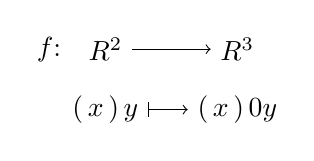
\begin{tikzpicture}[node distance=1mm]
        \node (functionName) at (0, 0) {$f$:};
        \node[right = of functionName] (domain) {$R^2$};
        \node[right = 1cm of domain] (codomain) {$R^3$};
        \node[below = 2mm of domain] (element) {$\begin{pmatrix}
                x \\
                y
            \end{pmatrix}$};
        \node at (element-|codomain) (image) {$\begin{pmatrix}
                x \\
                0 \\
                y
            \end{pmatrix}$};
        \draw[->] (domain) -- (codomain);
        \draw[|->] (element) -- (image);
    \end{tikzpicture}
\end{minipage}
\hfill
\begin{minipage}{0.35\linewidth}
    \begin{enumerate}[label=\protect\circled{\arabic*}]
        \item $f \in \mathcal{L}(R^2,R^3) ?$
        \item Kerf = ?
        \item Imf = ?
    \end{enumerate}
\end{minipage}
\begin{enumerate}[label=\protect\circled{\arabic*}]
    \item Necessary condition: $f(0_{E}) = 0_{F}$ : 
    $f(0_{R^2}) = \begin{pmatrix} 0 \\ 0 \end{pmatrix} 
    \rightarrow \begin{pmatrix} 0 \\ 0 \\ 0 \end{pmatrix}$ ?
    \[\forall (\alpha, X, Y) \in \mathbb{R} \times  \mathbb{R}^2 \times \mathbb{R}^2, X = \begin{pmatrix} x \\ y \end{pmatrix} \text{ and } Y = \begin{pmatrix} x' \\ y' \end{pmatrix}, x,y,x',y' \in \mathbb{R}\]
    \[f(\alpha \cdot X + Y) = \begin{pmatrix} \alpha \cdot x + x' \\ \alpha \cdot y + y' \end{pmatrix} = \begin{pmatrix} \alpha \cdot x + x' \\ 0 \\ \alpha \cdot y + y' \end{pmatrix} = \alpha \cdot \begin{pmatrix} x \\ 0 \\ y \end{pmatrix} + \begin{pmatrix} x' \\ 0 \\ y' \end{pmatrix} = \alpha \cdot f(X) + f(Y)\]
    so \circled{1} $f \in \mathcal{L}(R^2,R^3)$ \checkmark
    \item $Ker(f) = \left\{ \begin{pmatrix} x \\ y \end{pmatrix} \in R^2, \begin{pmatrix} x \\ 0 \\ y \end{pmatrix} = \begin{pmatrix} 0 \\ 0 \\ 0 \end{pmatrix} \right\} = \left\{ \begin{pmatrix} 0 \\ 0 \end{pmatrix} \right\}$
    \item $Im(f) = \left\{ \begin{pmatrix} x \\ 0 \\ y \end{pmatrix}, (x,y) \in R^2 \right\} = \left\{ x \begin{pmatrix} 1 \\ 0 \\ 0 \end{pmatrix} + y \begin{pmatrix} 0 \\ 0 \\ 1 \end{pmatrix}, (x,y) \in R^2 \right\}$ 
    \\$Im(f) = span\left\{ \begin{pmatrix} 1 \\ 0 \\ 0 \end{pmatrix}, \begin{pmatrix} 0 \\ 0 \\ 1 \end{pmatrix} \right\}$
\end{enumerate}
\subsection{Proposition}
\begin{enumerate}
    

    \item Let $f \in \mathcal{L}(E,F)$ and $g \in \mathcal{L}(F,G)$. Then: \[g \circ f \in \mathcal{L}(E,G)\]
    \item If $f$ is bijectif then $f{^{-1}}$ is bijective and $f{^{-1}} \in \mathcal{L}(F,E)$
    \item $\mathcal{L}(E,F)$ is a $\mathbb{K}-VS$:
        \newline
        \begin{minipage}{0.40\linewidth}
            
            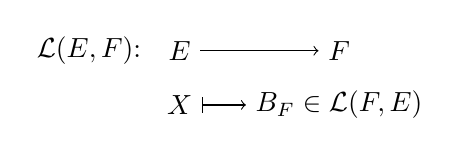
\begin{tikzpicture}[node distance=1mm]
                \node (functionName) at (0, 0) {$\mathcal{L}(E,F)$:};
                \node[right = of functionName] (domain) {$E$};
                \node[right = 1.5cm of domain] (codomain) {$F$};
                \node[below = 2mm of domain] (element) {$X$};
                \node at (element-|codomain) (image) {$B_F \in \mathcal{L}(F,E)$};
                \draw[->] (domain) -- (codomain);
                \draw[|->] (element) -- (image);
            \end{tikzpicture}
        \end{minipage}
        \hfill
        \begin{minipage}{0.59\linewidth}
            \begin{align*}
                \forall (\alpha, f, g) \in \mathbb{K} \times &\mathcal{L}^2(E,F) \\
                \alpha \cdot f + g \in &\mathcal{L}(E,F)
            \end{align*}
        \end{minipage}
    \item Let $f \in \mathcal{L}(A,B)$:
        \begin{itemize}
            \item $f$ is injective $ \Longleftrightarrow  Ker(f) = \left\{ 0_A \right\}$
            \item $f$ is surjective $ \Longleftrightarrow  Im(f) = B$
        \end{itemize}
\end{enumerate}
\section{Projects and Symmetries}
\subsection{Reminder:}
\subsubsection{Definition of supllementary subspaces}
Let $E$ a $\mathbb{K}$ - VS. Let $F$ and $G$ two supllementary $\mathbb{K}$ - VSS of $E$:
\[E = F \oplus G  \Longleftrightarrow \forall X \in E, \exists ! (X_F, X_G) \in F \times G, X = X_F + X_G\]
\subsection{Proposition}
\begin{tikzpicture}[node distance=1mm]
    \node (Let) at (-2, 0) {Let us consider:};
    \node (functionName) at (2, -0.5) {$p:$};

    \node[above right = -0.3cm and 0.5cm of functionName] (domain) {$E$};
    \node[right = 1.5cm of domain] (codomain) {$F$};
    \node[right = 0.1mm of codomain] (Rcodomain) {$\color{green} \subset E$};
    \draw [decorate, decoration={brace, mirror, raise=2.5pt}, green] (codomain.south west) -- (Rcodomain.south east) node [green, midway,sloped,below = 0.15cm] {\tiny $E$};
    \node[below = 5mm of domain] (element) {$X$};
    \node at (element-|codomain) (image) {$X_F$};
    \node[right = 1cm of image] (Rimage) {$\color{green} X_F$};
    \draw[->] (domain) -- (codomain);
    \draw[green, |->] (image) -- (Rimage) node[midway, above]{$\color{green} p$};
    \draw[|->] (element) -- (image) node[midway, above]{$\color{green} p$};
\end{tikzpicture}
\begin{enumerate}
    \item $p \in \mathcal{L}(E)$
    \item $p \circ p$ $(=p^2) = p$
    \item \begin{itemize}
        \item $Ker(p) = G$
        \item $Im(p) = F$
    \end{itemize}
\end{enumerate}
\subsection{Definition}
We call projector from $\mathbb{K}$ - VS $E$ over $\mathbb{K}$ - VS $F$, any endomorphism $p$ of $E$ such that $p \circ p = p$. (We often say that $p$ is a projector over $F$ parallel of/alongside $G$.) 
\[Im(p) \oplus Ker(p) = E\]

\begin{tikzpicture}[node distance=1mm]
    \node (Let) at (-2, 0) {Let us consider:};
    \node (functionName) at (2, -0.5) {$S:$};

    \node[above right = -0.3cm and 0.5cm of functionName] (domain) {$E$};
    \node[right = 3cm of domain] (codomain) {$E$};
    \node[below = 5mm of domain] (element) {$X$};
    \node at (element-|codomain) (image) {$(2P - Id_E)(X)$};
    \node[right = -0.1cm of image] (Rimage) {$\color{green} = 2p(x)-X$};
    \draw[->] (domain) -- (codomain);
    \draw[|->] (element) -- (image);
\end{tikzpicture}

\begin{minipage}{0.4\linewidth}    
    \begin{enumerate}
        \item $S \in \mathcal{L}(E)$
        \item $\forall X \in E, S(X) = X_E - X_G$
        \item $S \circ S = Id_E$
    \end{enumerate}
\end{minipage}
\hfill
\begin{minipage}{0.4\linewidth} 
    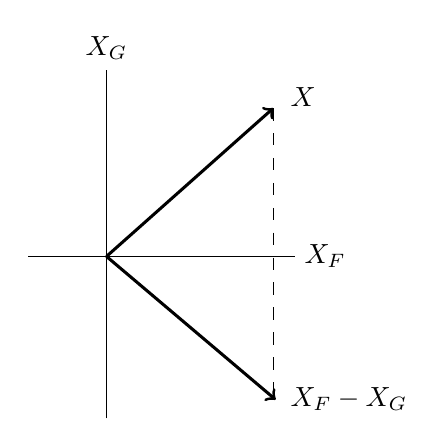
\begin{tikzpicture}[x=0.75pt,y=0.75pt,yscale=-1,xscale=1]
        %Straight Lines [id:da24929647938311184] 
        \draw    (189.3,210) -- (189.3,42.05) node[above] {$X_G$};
        %Straight Lines [id:da4428013785785254] 
        \draw    (151.6,132) -- (280,132) node[right] {$X_F$};
        %Straight Lines [id:da03148052252332034] 
        \draw[->,line width=1.1pt]  (189.3,132) -- (269.7,60.55) ;
        %Straight Lines [id:da8135470928175486] 
        \draw[->,line width=1.1pt]    (189.3,132) -- (270.8,201) ;
        %Straight Lines [id:da10546756418707193] 
        \draw [dash pattern={on 4.5pt off 4.5pt}]  (269.7,60.55) -- (269.7,157.55) -- (269.7,200.05) ;
        
        % Text Node
        \draw (276.7,49.2) node [anchor=north west][inner sep=0.75pt]    {$X$};
        % Text Node
        \draw (276.7,193.7) node [anchor=north west][inner sep=0.75pt]    {$X_F-X_G$};
    \end{tikzpicture} 
\end{minipage}
\section{Rank Nullity Theorem (RNT)}
\subsection{Definition of Rank}
Let $E$ and $F$ two finite dimensional vector spaces. We call rank of any mapping $f$ from $\mathcal{L}(E,F)$ and denote $rank(f)$ the dimension of $Im(f)$: \[rank (f) = dim (Im(f))\]
\subsection{Proposition}
Let $E$ a finite dimensional $\mathbb{K}$ - VS such that $B = (U_1, U_2, \dots, U_n)$ a basis of $E$. Let $F$ a $\mathbb{K}$ - VS.
Then let $f \in \mathcal{L}(E,F)$.
We have: \[Im (f) = sp(\{f(U_1), f(U_2), \dots, f(U_n)\})\]
We then deduce the following theorem: 
\subsection{Theorem (Rank Nullity Theorem)} 
Let $E$ a finite dimensional VS and $f \in \mathcal{L}(E,F)$. Then: \\
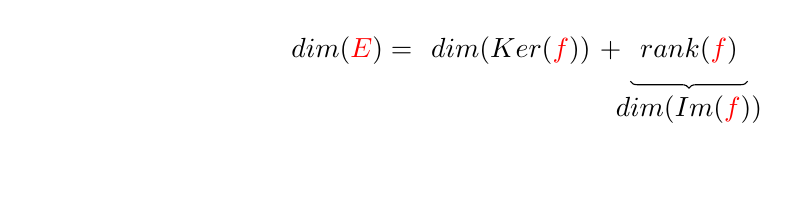
\begin{tikzpicture}
    \node (Let) at (-2, 0) {};
    \node (E) at (2, 1.5) {$dim(\color{red}E\color{black}) = $};
    \node[right = -0.1mm of E] (kern) {$dim(Ker(\color{red}f\color{black}))$ $ + $};
    \node[right = -0.1mm of kern] (rank) {$rank(\color{red}f\color{black})$};
    \draw [decorate, decoration={brace, mirror, raise=2.5pt}] (rank.south west) -- (rank.south east) node [midway,sloped,below = 0.15cm] {$dim(Im(\color{red}f\color{black}))$};
\end{tikzpicture}
\subsection{Corollary}
Let $f \in \mathcal{L}(E,F)$ where $E$ and $F$ two finite dimensional vector spaces.
\[\text{If } dim(E) = dim(F) (\Longleftrightarrow dim(Ker(f)) = 0 \text{ or } dim(Im(f)) = 0)\]
\[\Longrightarrow\]
\[\text{f injective} \Longleftrightarrow \text{f surjective} \Longleftrightarrow \text{f bijective}\]
\subsection{Involvement}
\[\text{f injective} \Longleftrightarrow Ker(f) = \left\{ 0_E \right\}\]
\[\left[ \text{f injective} \Longrightarrow dim(E) \le dim(F) \right] \Longleftrightarrow \left[ dim(E) > dim(F) \Longrightarrow \text{f not injective} \right]\]
\[\text{f surjective} \Longleftrightarrow Im(f) = F\]
\[\left[ \text{f surjective} \Longrightarrow dim(E) \ge dim(F) \right] \Longleftrightarrow \left[ dim(E) < dim(F) \Longrightarrow \text{f not surjective} \right]\]
\subsection{Proof of corollary}
Hypothesis: $dim(E) = dim(F)$ 
\begin{align*}
\text{f injective} &\Longleftrightarrow Ker(f) = \left\{ 0_E \right\} \\
&\Longleftrightarrow dim(Ker(f)) = 0 \\
&\Longleftrightarrow dim(E) = dim(Ker(f)) + dim(Im(f)) \\
&\Longleftrightarrow dim(E) = dim(Im(f)) \\
&\Longleftrightarrow dim(F) = dim(Im(f)) \\
\text{f surjective} &\Longleftrightarrow Im(f) = F 
\end{align*}
\section{Important Proof}
\fbox{
\begin{minipage}{0.9\linewidth}   
    \subsection{Proposition (Kernel and image).}
    Let $E$ and $F$ be two vector spaces over $\mathbb{R}$ and $f \in \mathcal{L}(E,F)$.
    \begin{enumerate}
        \item $Ker(f)$ is a linear subspace of $E$.
        \item $Im(f)$ is a linear subspace of $F$.
    \end{enumerate}
\end{minipage}}
\subsubsection{Proof:}
\begin{enumerate}
    \item $Ker(f)$ is a linear subspace of $E$.
    \begin{itemize}
        \item By definition, $Ker(f) \subset E$. Since $f$ is a linear map from $E$ to $F$, we know that $f(0_E) = 0_F$ , that is, $0_E \in Ker(f)$.
        \item Let $(u, v) \in (Ker(f))^2$ and $\alpha \in \mathbb{R}$.
        \begin{align*}
            f(\alpha u + v) &= \alpha f(u) + f(v) \text{ because } f \text{ is a linear map} \\
            &= \alpha (0_F) + (0_F) \\
            &= 0_F
        \end{align*}
        Thus, $\alpha u + v \in Ker(f)$. $Ker(f)$ is hence a linear subspace of $E$.
    \end{itemize}
    \item $Im(f)$ is a linear subspace of $F$.
    \begin{itemize}
        \item By definition, $Im(f) \subset F$. Since $f$ is a linear map from $E$ to $F$, we know that $0_F = f(0_E)$. Thus, $0_F \in Im(f)$.
        \item Let $(v, v') \in (Im(f))^2$ and $\alpha \in \mathbb{R}$. Then:
        \[v \in Im(f) \Leftrightarrow \exists w \in E, v = f(w) \quad \text{and} \quad v' \in Im(f) \Leftrightarrow \exists w' \in E, v' = f(w')\]
        We hence get:
        \begin{align*}
            \alpha v + v' &= \alpha f(w) + f(w') \\
            &= f(\alpha w + w) \text{ since } f \text{ is a linear map}\\
        \end{align*}
        This proves that $\alpha v + v' \in Im(f)$. $Im(f)$ is hence a linear subspace of $F$.
    \end{itemize}
\end{enumerate}
\fbox{
\begin{minipage}{0.9\linewidth}   
    \subsection{
        Proposition (Characterizing injective and surjective linear maps).}
    Let $E$ and $F$ be two vector spaces over $\mathbb{R}$ and $f \in \mathcal{L}(E,F)$.
    \begin{enumerate}
        \item $f$ is injective if and only if $Ker(f) = \left\{ 0_E \right\}$.
        \item $f$ is surjective if and only if $Im(f) = F$.
    \end{enumerate}
\end{minipage}}
\subsubsection{Proof:}
\begin{enumerate}
    \item \fbox{$\Longrightarrow$} Assume that $f$ is injective. We hence know that
    \[ \forall (u, u') \in E ^2, f(u) = f(u') \Rightarrow u = u'\]
    \begin{itemize}
        \item Let $u \in Ker(f)$. \\
        $f(u) = 0_F$ and $0_F = f(0_E)$. (because $f$ is a linear map) $\Rightarrow f(u) = f(0_E) \Rightarrow u = 0_E$ using the injectivity definition.
        This proves that $Ker(f) \subset \left\{ 0_E \right\}$.
        \item Since $\left\{ 0_E \right\} \subset Ker(f)$, we get $Ker(f) = \left\{ 0_E \right\}$.
    \end{itemize}
    \fbox{$\Longleftarrow$} Assume that $Ker(f) = \left\{ 0_E \right\}$. \\
    Let $(u, u') \in E ^2$ such that $f(u) = f(u')$. Then
    \begin{align*}
        f(u) = f(u') &\Rightarrow f(u) - f(u') = 0_F \\
        &\Rightarrow f(u - u') = 0_F \text{ because } f \text{ is a linear map} \\
        &\Rightarrow u - u' \in Ker(f)\\
        &\Rightarrow u - u' = \left\{ 0_E \right\} \text{ because } Ker(f) = \left\{ 0_E \right\} \\
        &\Rightarrow u - u' = 0_E \\
        &\Rightarrow u = u' 
    \end{align*}
    $f$ is hence injective.
    \item For the surjectivity, we have:
    \begin{align*}
        f \text{ surjective} &\Longleftrightarrow \forall v \in F, \exists u \in E, v = f(u) \\
        &\Longleftrightarrow \forall v \in F, v \in Im(f) \\
        &\Longleftrightarrow F \subset Im(f) \\
        &\Longleftrightarrow Im(f) = F \text{ since the inclusion } Im(f) \subset F \text{ is always true}
    \end{align*}
\end{enumerate}
\end{document}